\documentclass[11pt,fleqn]{article}
%\usepackage{CJK}
\usepackage{latexsym}
\usepackage{color}
\usepackage{graphicx, float}\usepackage{graphicx}
\usepackage{algorithmic}
\usepackage{algorithm}
%\usepackage{algpseudocode}
%\usepackage[colorlinks]{hyperref}
\usepackage[toc,page]{appendix}
\usepackage{bm}
\setlength{\oddsidemargin}{-0.0in}
\setlength{\evensidemargin}{-0.0in} \setlength{\textwidth}{6.0in}
\setlength{\textheight}{9.0in} \setlength{\topmargin}{-0.2in}
%\usepackage[boxruled]{algorithm2e}

%\setlength{\leftmargin}{0.7in}
\usepackage{amssymb, graphicx, amsmath}  %  fancyheadings,
\usepackage{setspace}
\newcommand\qed{\qquad $\square$}
\newcommand{\nn}{\nonumber}

\def \[{\begin{equation}}
\def \]{\end{equation}}
\def\proof{{\bf Proof:\quad}}
\def \endzm {\quad $\Box$}
\def\dist{\hbox{dist}}

\usepackage{tabularx,booktabs}
\newcolumntype{C}{>{\centering\arraybackslash\hsize=.5\hsize}X} % centered version of "X" type
\setlength{\extrarowheight}{1pt}
\usepackage{caption}% <-- added


\newcommand{\R}{\mathbb{R}}
%\newtheorem{yinli}{����}[section]
\newcommand{\D}{\displaystyle}
\newcommand{\T}{\textstyle}
\newcommand{\SC}{\scriptstyle}
\newcommand{\FT}{\footnotesize}

\usepackage{hyperref}
\newcommand\fnurl[2]{%
  \href{#2}{#1}\footnote{\url{#2}}%
}


%\newtheorem{theorem}{Theorem}[section]
%\renewcommand{\thetheorem}{\arabic{section}.\arabic{theorem}}
\newtheorem{definition}{Definition}
\renewcommand{\thedefinition}{\arabic{section}.\arabic{definition}}
\newtheorem{lemma}{Lemma}[section]
\renewcommand{\thelemma}{\arabic{section}.\arabic{lemma}}
\newtheorem{remark}{Remark}
\renewcommand{\theremark}{\arabic{section}.\arabic{remark}}
\newtheorem{proposition}{Proposition}[section]
\renewcommand{\theproposition}{\arabic{section}.\arabic{proposition}}
\newtheorem{corollary}{Corollary }[section]
\renewcommand{\thecorollary}{\arabic{section}.\arabic{corollary}}
\renewcommand{\theequation}{\arabic{section}.\arabic{equation}}
\renewcommand{\baselinestretch}{1.35}
\newtheorem{exam}{Example}[section]
\renewcommand{\theexam}{\arabic{section}.\arabic{exam}}
\newtheorem{theo}{Theorem}[section]
\renewcommand{\thetheo}{\arabic{section}.\arabic{theo}}
\begin{document}
%\begin{CJK*}{GBK}{song}

\begin{center}

{\LARGE \bf CS391L Machine Learning HW4: Gaussian Process}\\

\vskip 25pt
 {Zeyuan Hu, iamzeyuanhu@utexas.edu }\\
\vskip 5pt
{\small EID:zh4378 Fall 2017 }

\end{center}

\begin{spacing}{1.5}
\section{Introduction}

\paragraph{}In this task, we study the human movement position data captured by the motion 
capture system. We want to measure the stiffness of the movement, which happens when humans 
co-contract opposing muscles to move. One hypothesis is that if a joint controller is stiff,
it will produce reliable repeated movements, whereas if it is very loose, there will be more
variation in repeated movements. We use the Gaussian Process (GP) to test this hypothesis
and we find out that GP in general is a good model to measure the human stiffness and thus we
are able to confirm the hypothesis.

This writeup is organized in the following way: In the first section, I will 
describe the steps to finish the task. Next, I will talk about the experimentation result. 
Lastly, I will give a breif summary of the whole work.

\section{Method}

\subsection{Gaussian Process}

In GP, we put a probability distribution over the space of functions, which can be specified by
the mean and covariance functions. Concretely, GP is described
as a function $G(k(\boldsymbol{x}, \boldsymbol{x'}))$ that models some underlying functin $f(\boldsymbol{x})$.
The covariance function $k(\boldsymbol{x}, \boldsymbol{x'})$ gives us the expected covariance matrix
between the values of $f$ at $\boldsymbol{x}$ and $\boldsymbol{x'}$. In this task, we use the squared exponential covariance matrix
(also called Gaussian kernel or RBF kernel).

$$
k(\boldsymbol{x}, \boldsymbol{x'}) = \exp(\sigma_f) \exp(-\frac{1}{2}\exp(\sigma_l)\left|\boldsymbol{x} -\boldsymbol{x'}\right|^2)
+ \exp(\sigma_n) \boldsymbol{I}
$$

\noindent where the signal variance $\sigma_f^2$ controls the overall variance of the function, and the length scale $\sigma_l$ changes
the degree of smoothing, trading it off against how well the curve matches the training data. $\sigma_n$ expresses how much noise
is expected in the data points. Those are the hyperparameters that we will explore in detials in the experiment section. 

To apply GP to the gression task, we perform the following steps: we compute the covariance matrix of the training data, and also
the covariances between the training and test data, and the test data alone. Then we compute the mean and covariance of the 
posterior distribution and sample from it. The detailed steps is the following:

For given training data $(\boldsymbol{X}, \boldsymbol{t})$, where $\boldsymbol{x}$ is the vector of training time points and 
$\boldsymbol{t}$ is the vector of corresponding training function values at the respective time points. We have test data $\boldsymbol{x^*}$,
covariance function $k()$, and hyperparameters $\boldsymbol{\theta} = (\sigma_f^2, \sigma_l^2, \sigma_n^2)$:

\begin{itemize}
\item Compute the covariance matrix $\boldsymbol{K} = k(\boldsymbol{X}, \boldsymbol{X}) + \sigma_n \boldsymbol{I}$
\item Compute the covariance matrix $\boldsymbol{k^*} = k(\boldsymbol{X}, \boldsymbol{x^*})$
\item Compute the covariance matrix $k^{**} = k(\boldsymbol{x^*}, \boldsymbol{x^*})$
\item The mean of the process is $\boldsymbol{{k^*}^T}\boldsymbol{K}^{-1}\boldsymbol{t}$
\item The covariance is $k^{**} - \boldsymbol{{k^*}^T}\boldsymbol{K}^{-1}\boldsymbol{k^*}$
\end{itemize}

The new point $x_i^*$ will be interpolated with a gussian with mean $m_i$ and variance $\text{Cov}_{i,i}$. Thus, if 
we want to build a 95\% confidence interval over the interpolated $m_i$ value for $x_i^*$, we will have an upper bound
of $m_i + 1.96\sqrt{(\text{Cov}_{i,i}}$ and a lower bound of $m_i - 1.96\sqrt{\text{Cov}_{i,i}}$, where 1.96 is the z-score
for 95\% confidence.

As we will see in the experiment section, hyperparameters $\boldsymbol{\theta} = (\sigma_f^2, \sigma_l^2, \sigma_n^2)$
will have a significant effect on the shape of the resulting output curve. Thus, finding the correct hyperparameters
is very important. One way is to choose the hyperparameters that maximize the log probability of seeing the data, which is
specified by

$$
\log P(\boldsymbol{t}|\boldsymbol{x}, \boldsymbol{\theta}) = -\frac{1}{2}\boldsymbol{t}^T(\boldsymbol{K} + \sigma_n^2\boldsymbol{I})^{-1}
\boldsymbol{t} - \frac{1}{2}\log\left|\boldsymbol{K} + \sigma_n^2 \boldsymbol{I}\right| - \frac{N}{2}\log 2\pi
$$

\noindent We can use the gradient descent method to minimize this log likelihood. The only thing we need is the gradient. We let
$\boldsymbol{Q} = (\boldsymbol{K} + \sigma_n^2\boldsymbol{I})$ and since $\boldsymbol{Q}$ is a function of all
of the hyperparameters $\boldsymbol{\theta}_i$. Then the gradient is computed as

$$
\frac{\partial}{\partial \boldsymbol{\theta}}\log P(\boldsymbol{t}|\boldsymbol{x},\boldsymbol{\theta}) 
= \frac{1}{2}\boldsymbol{t}^T\boldsymbol{Q}^{-1}\frac{\partial \boldsymbol{Q}}{\partial\boldsymbol{\theta}} \boldsymbol{Q}^{-1}\boldsymbol{t}
- \frac{1}{2}\text{trace}(\boldsymbol{Q}^{-1}\frac{\partial \boldsymbol{Q}}{\partial \boldsymbol{\theta}})
$$

\noindent Since we are using the squared exponetial covariance function, then $\frac{\partial \boldsymbol{Q}}{\partial\boldsymbol{\theta}}$
is equal to

\begin{eqnarray*}
\frac{\partial k}{\sigma_f} &=& k' \\
\frac{\partial k}{\sigma_l} &=& k' \times (-\frac{1}{2}\exp(\sigma_l)\left|\boldsymbol{x}-\boldsymbol{x'}\right|^2) \\
\frac{\partial k}{\sigma_n} &=& \exp(\sigma_n)\boldsymbol{I} \\
\end{eqnarray*}

\noindent where $k(x,x') = k' + \exp(\sigma_n)\boldsymbol{I}$.

\subsection{Work with the data} \label{work with the data}

In this task, we have 12 subjects' motion capture data and thus there are 12 directories (i.e., AG, CJ, CT, etc.).
Each directory contains five subdirectories, which means that each subject traced a curve 5 times. In each subdirectory,
there is a csv file. Totally there are 50 markers (sensors), and each marker has position (x,y,z). Thus, the marker
positions are presented as (markerIndex\_x, markerIndex\_y, markerIndex\_z). For example the position of marker 6 is
(5\_x, 5\_y, 5\_z). There are C-labeled data associated with each marker indicating whether the marker position is valid or not.
If the motion capture system cannot get the marker positions, then the corresponding C-label value is negative. For example,
if the (5\_x, 5\_y, 5\_z, 5\_c) is (1, 1.2, 1.3, 3), then the recording position is useful. However, if the tuple is (1, 1.2, 1.3, -1),
then the recording position is useless.

\subsection{Implementation}

We utilize the scikit-learn package to perform the gaussian process hyperparameters learning and regression \cite{scikit-learn}.  
The whole implementation can be break down into two parts: the data processing and the GP. For the data processing part,
we use \verb|generate_observed_data_list| to read in the csv files under the \verb|'data_GP/'| directory. Here we use \verb|one_subject|
variable to control whether we want to read all the csv files associated with one specific subject or we want to read in
all the csv files. Once we read in the csv files, we invoke \verb|read_in_data| function to process the csv files by formating
all the x-coordinate values, y-coordinate values, and z-coordinate values into matrices with dimension $50\times1030$. Then we check
the C-label value to remove invalid data entries and append the result values as a list into \verb|x_clean|, \verb|y_clean|, and 
\verb|z_clean| correspondingly. The dimension of all those three variables are $50\times\text{number of timeframe with valid data}$.

For the GP part, the key is to construct the kernel with the hyperparameters we discuss previously and whether we fix our hyperparameters
or not. We use \verb|ConstantKernel| (i.e., \fnurl{ConstantKernel API}{http://scikit-learn.org/stable/modules/generated/sklearn.gaussian_process.kernels.ConstantKernel.html}) with parameter \verb|constant_value| to control $\sigma_f$. We use \verb|RBF| (i.e., \fnurl{RBF API}{http://scikit-learn.org/stable/modules/generated/sklearn.gaussian_process.kernels.RBF.html}) with \verb|length_scale| to control $\sigma_l$. Lastly, we \verb|WhiteKernel| (i.e., \fnurl{WhiteKernel API}{http://scikit-learn.org/stable/modules/generated/sklearn.gaussian_process.kernels.WhiteKernel.html}) to control $\sigma_n$.

\section{Results}

We first plot the GP model fitting one marker of one trail. We pick $x_0$ marker in the first movement data of the subject
"AG". We make a comparison between fitting one marker of one trail with fixed hyperparameters $\sigma_f = 1.0$, $\sigma_l = 10$,
and $\sigma_n = 10^{-2}$ and the fitting with the learned hyperparameters. In this case, the hyperparameters
are optimized as $\sigma_f = 0.487^2$, $\sigma_l = 41$, and $\sigma_n = 10^{-10}$. Figure 1 and Figure 2 show the comparison
result.

\begin{figure}
\centering
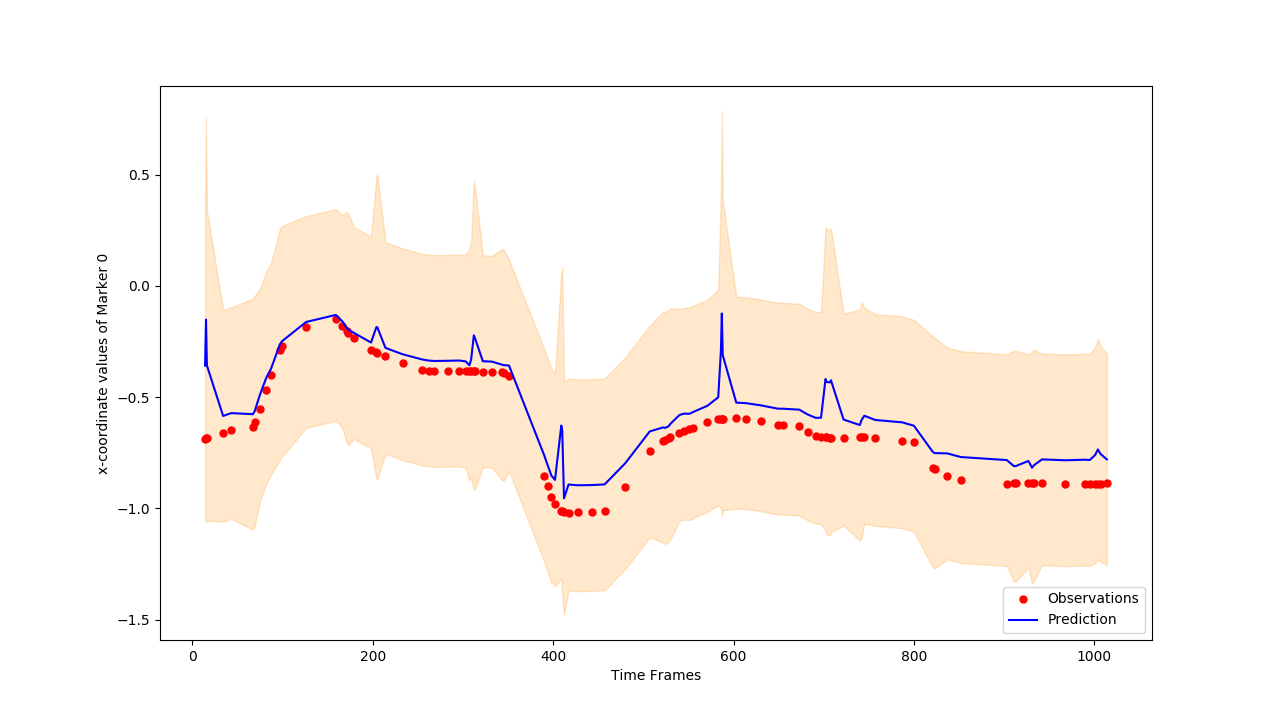
\includegraphics[scale=0.5]{param_fix.png} 
\caption{Initial, bad hyperparameters}
\end{figure}

\begin{figure}
\centering
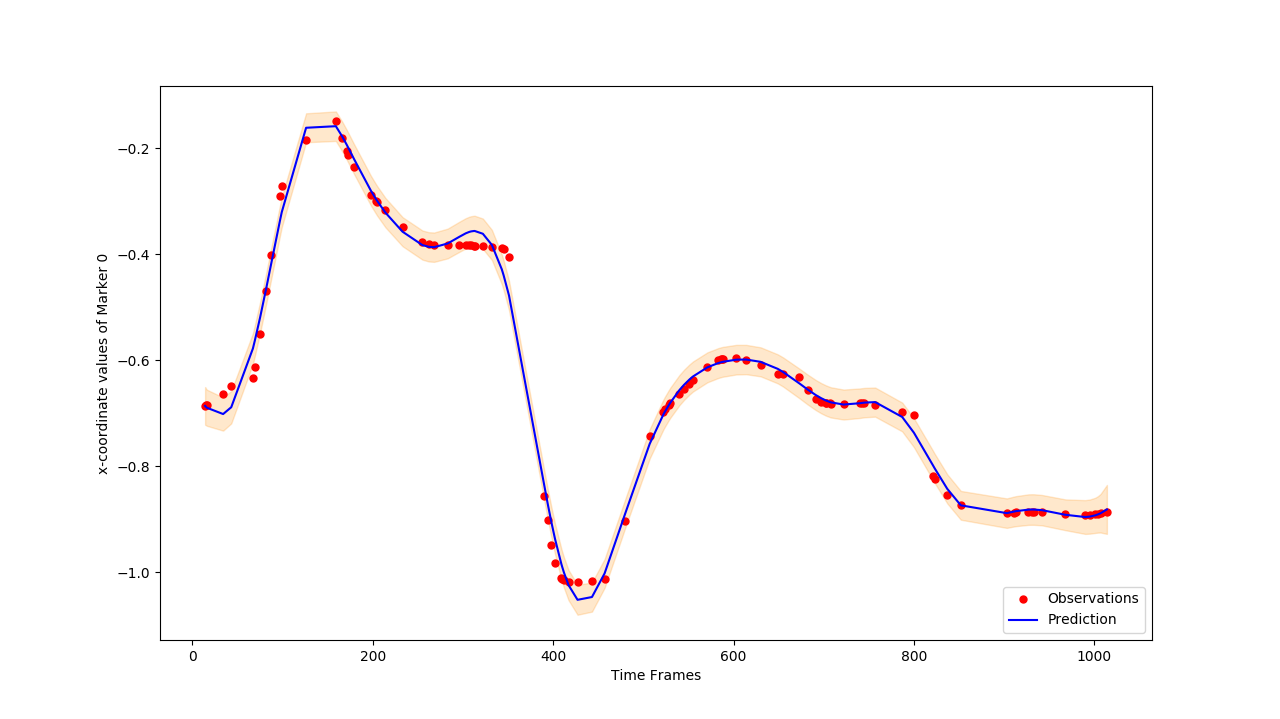
\includegraphics[scale=0.5]{single_optimized.png} 
\caption{Initial, bad hyperparameters}
\end{figure}

Next, we try to vary the hyperparameters across the data traces. Our hypothesis is that if a joint
controller is stiff, it will produce reliable repeated movements, whereas if it is very loose, there
will be more variation in repeated movements. Table 1 summarizes the optimized hyperparameters for 
the selected subjects. Figure 4 and Figure 5 plot all five repeated movements data for subject "AG" and 
subject "YY". I randomly select one movement data of all five momement data of a subject to fit the 
gaussian process and see if the resulting model can describe all five movement data relative well.

\begin{table}[!htb]
\captionsetup{size=footnotesize}
\caption{Optimized hyperparameters for selected subjects} \label{tab:freq}
\setlength\tabcolsep{0pt} % let LaTeX compute intercolumn whitespace
\footnotesize\centering
%This table provides the frequencies.

\smallskip 
\begin{tabular*}{\columnwidth}{@{\extracolsep{\fill}}rccr}
\toprule
  Subject  & $\sigma_f$ & $\sigma_l$ & $\sigma_n$ \\
\midrule
 YY & $0.404^2$   & $36.7$    & $10^{-10}$      \\
 AG & $0.487^2$   & $41$    & $10^{-10}$     \\
 CJ & $0.393^2$   & $40.1$    & $1.15\times10^{-10}$     \\
 CT & $0.206^2$   & $20.1$    & $10^{-10}$     \\
 EK & $0.257^2$   & $62$    & $1.6\times10^{-10}$     \\
\bottomrule
\end{tabular*}
\end{table}


\begin{figure}
\centering
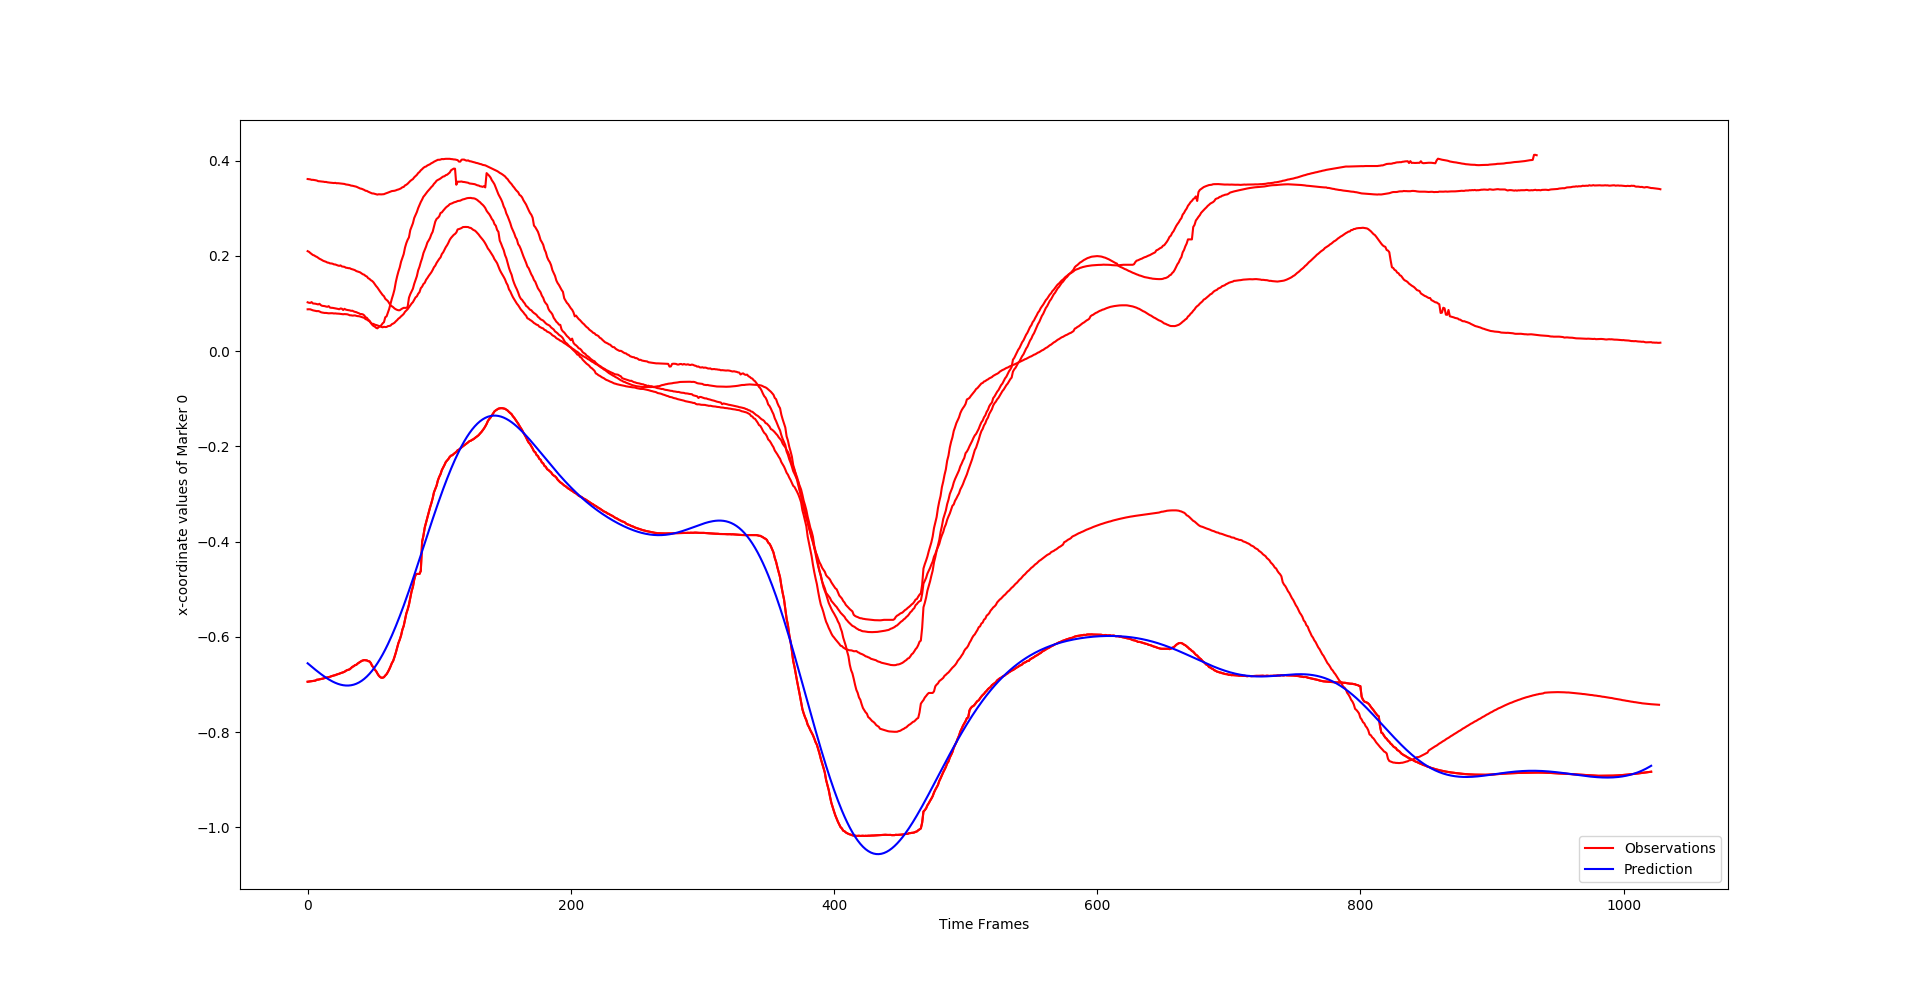
\includegraphics[scale=0.4]{AG.png} 
\caption{Plot of movement data of subject "AG"}
\end{figure}

\begin{figure}
\centering
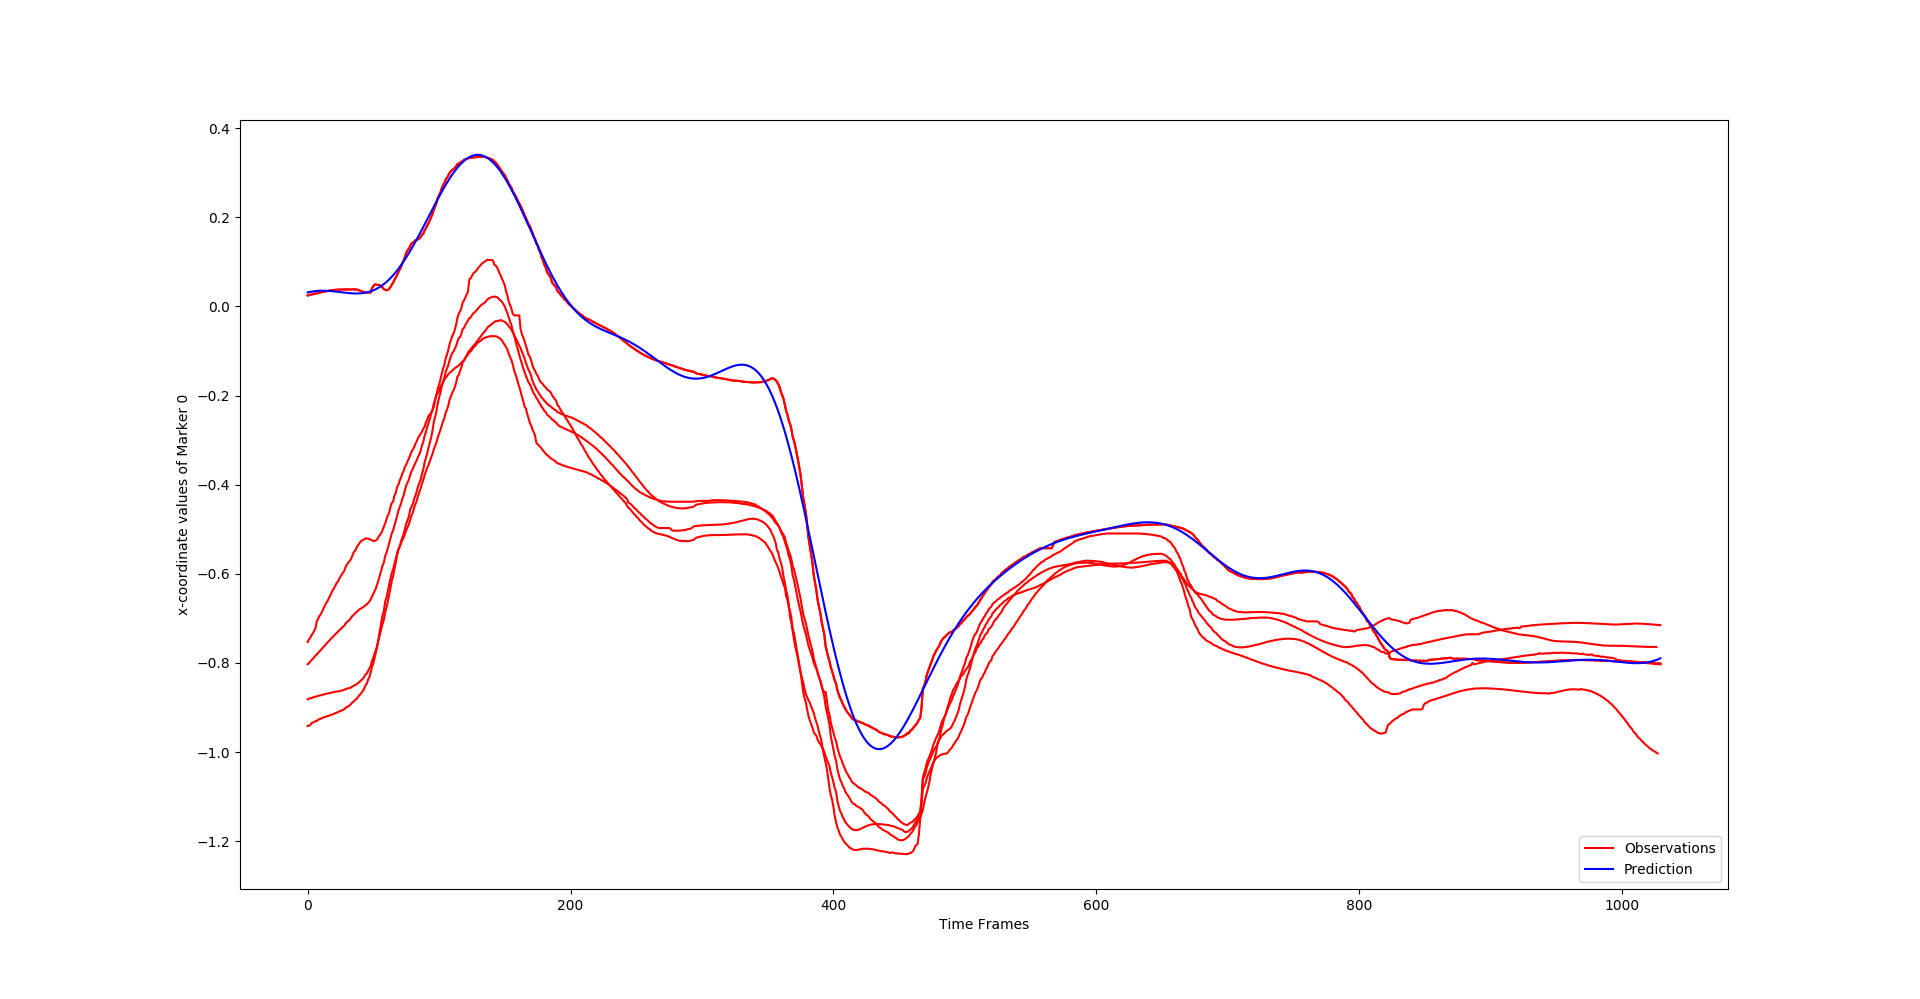
\includegraphics[scale=0.4]{YY.png} 
\caption{Plot of movement data of subject "YY"}
\end{figure}

It can be seen that the variation across all repeated movements for both "AG" and for "YY" 
are relative small. This indicates that joint controller
for both "AG" and "YY" is stiff.

Lastly, I fit the trails over all the subjects. The result is shown in Figure 5. 

\begin{figure}
\centering
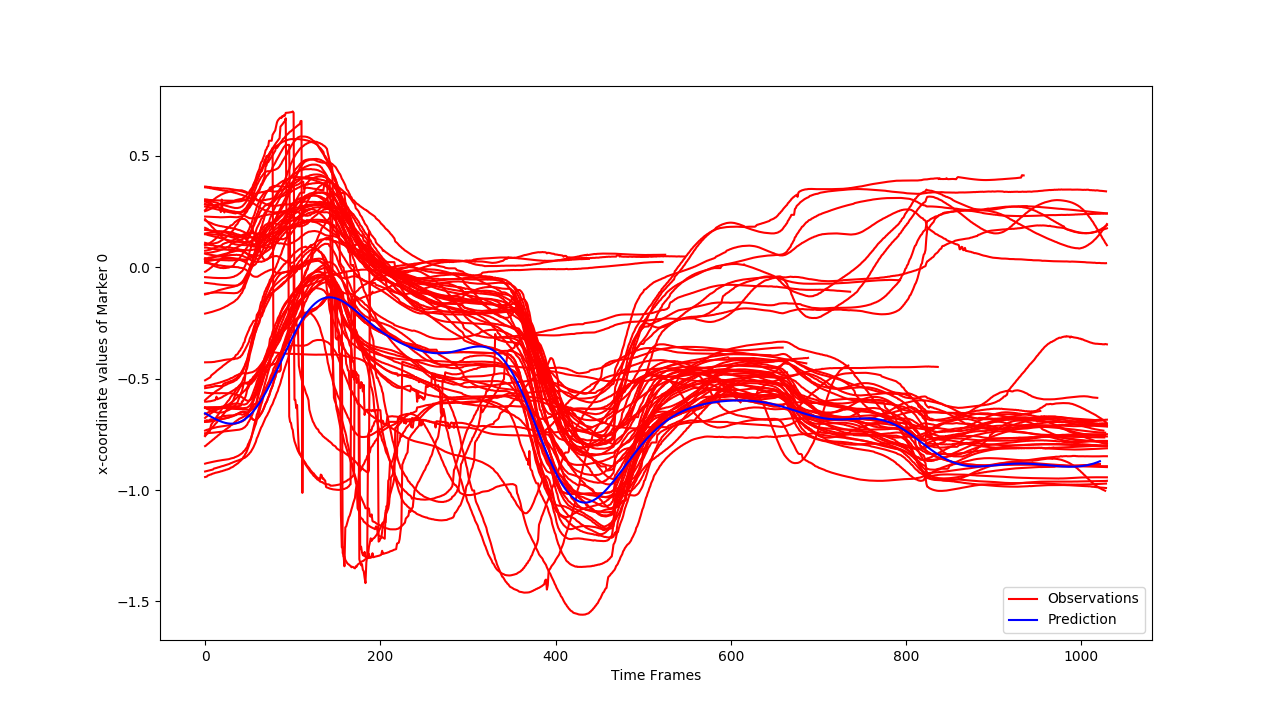
\includegraphics[scale=0.4]{multi_optimized.png} 
\caption{use the GP fitting trails over subjects on Marker 0\_x}
\end{figure}

\section{Summary}

In this task, I apply the gaussian process regression to the human movement position data
and find out that the joint controller for the subjects are stiff. In addition, I tune 
the hyperparameters in order to get the good fit of the model to the data.

\end{spacing}

\begin{appendices}

\section{How to run the code}

\paragraph{}To run my code, unzip the \verb|hw4.zip| and put the directory named \verb|data_GP| that 
contains data files under the same directory with \verb|gp.py|. Then, you
can run the code with the following commands:

\begin{itemize}
\item \verb|python gp.py S| Run the gaussian process regression on a single trail (i.e., x\_0)
\item \verb|python gp.py M| Run the gaussian prcoess regression on all the trails of all the subjects 
\item \verb|python gp.py SN| Run the gaussian process regression on a single trail (i.e., x\_0) and fix the hyperparameters
\item \verb|python gp.py SUB| Run the gaussian process regression on all trails of a single subject
\end{itemize}

My code is heavily commented and please take a look if there are any type of questions.

\end{appendices}

\bibliographystyle{ieeetr}
\bibliography{report}
\end{document}
